%%
%% Beginning of file 'sample61.tex'
%%
%% Modified 2016 September
%%
%% This is a sample manuscript marked up using the
%% AASTeX v6.1 LaTeX 2e macros.
%%
%% AASTeX is now based on Alexey Vikhlinin's emulateapj.cls 
%% (Copyright 2000-2015).  See the classfile for details.

%% AASTeX requires revtex4-1.cls (http://publish.aps.org/revtex4/) and
%% other external packages (latexsym, graphicx, amssymb, longtable, and epsf).
%% All of these external packages should already be present in the modern TeX 
%% distributions.  If not they can also be obtained at www.ctan.org.

%% The first piece of markup in an AASTeX v6.x document is the \documentclass
%% command. LaTeX will ignore any data that comes before this command. The 
%% documentclass can take an optional argument to modify the output style.
%% The command below calls the preprint style  which will produce a tightly 
%% typeset, one-column, single-spaced document.  It is the default and thus
%% does not need to be explicitly stated.
%%
%%
%% using aastex version 6.1
\documentclass[twocolumn]{aastex61}

%% The default is a single spaced, 10 point font, single spaced article.
%% There are 5 other style options available via an optional argument. They
%% can be envoked like this:
%%
%% \documentclass[argument]{aastex61}
%% 
%% where the arguement options are:
%%
%%  twocolumn   : two text columns, 10 point font, single spaced article.
%%                This is the most compact and represent the final published
%%                derived PDF copy of the accepted manuscript from the publisher
%%  manuscript  : one text column, 12 point font, double spaced article.
%%  preprint    : one text column, 12 point font, single spaced article.  
%%  preprint2   : two text columns, 12 point font, single spaced article.
%%  modern      : a stylish, single text column, 12 point font, article with
%% 		  wider left and right margins. This uses the Daniel
%% 		  Foreman-Mackey and David Hogg design.
%%
%% Note that you can submit to the AAS Journals in any of these 6 styles.
%%
%% There are other optional arguments one can envoke to allow other stylistic
%% actions. The available options are:
%%
%%  astrosymb    : Loads Astrosymb font and define \astrocommands. 
%%  tighten      : Makes baselineskip slightly smaller, only works with 
%%                 the twocolumn substyle.
%%  times        : uses times font instead of the default
%%  linenumbers  : turn on lineno package.
%%  trackchanges : required to see the revision mark up and print its output
%%  longauthor   : Do not use the more compressed footnote style (default) for 
%%                 the author/collaboration/affiliations. Instead print all
%%                 affiliation information after each name. Creates a much
%%                 long author list but may be desirable for short author papers
%%
%% these can be used in any combination, e.g.
%%
%% \documentclass[twocolumn,linenumbers,trackchanges]{aastex61}

%% AASTeX v6.* now includes \hyperref support. While we have built in specific
%% defaults into the classfile you can manually override them with the
%% \hypersetup command. For example,
%%
%%\hypersetup{linkcolor=red,citecolor=green,filecolor=cyan,urlcolor=magenta}
%%
%% will change the color of the internal links to red, the links to the
%% bibliography to green, the file links to cyan, and the external links to
%% magenta. Additional information on \hyperref options can be found here:
%% https://www.tug.org/applications/hyperref/manual.html#x1-40003

%% If you want to create your own macros, you can do so
%% using \newcommand. Your macros should appear before
%% the \begin{document} command.
%%
\newcommand{\vdag}{(v)^\dagger}
\newcommand\aastex{AAS\TeX}
\newcommand\latex{La\TeX}
\newcommand{\sm}{M_\odot}
\newcommand{\sr}{R_\odot}

%% Reintroduced the \received and \accepted commands from AASTeX v5.2
\received{\today}
\revised{}
\accepted{}
%% Command to document which AAS Journal the manuscript was submitted to.
%% Adds "Submitted to " the arguement.
\submitjournal{ApJ}

%% Mark up commands to limit the number of authors on the front page.
%% Note that in AASTeX v6.1 a \collaboration call (see below) counts as
%% an author in this case.
%
%\AuthorCollaborationLimit=3
%
%% Will only show Schwarz, Muench and "the AAS Journals Data Scientist 
%% collaboration" on the front page of this example manuscript.
%%
%% Note that all of the author will be shown in the published article.
%% This feature is meant to be used prior to acceptance to make the
%% front end of a long author article more manageable. Please do not use
%% this functionality for manuscripts with less than 20 authors. Conversely,
%% please do use this when the number of authors exceeds 40.
%%
%% Use \allauthors at the manuscript end to show the full author list.
%% This command should only be used with \AuthorCollaborationLimit is used.

%% The following command can be used to set the latex table counters.  It
%% is needed in this document because it uses a mix of latex tabular and
%% AASTeX deluxetables.  In general it should not be needed.
%\setcounter{table}{1}

%%%%%%%%%%%%%%%%%%%%%%%%%%%%%%%%%%%%%%%%%%%%%%%%%%%%%%%%%%%%%%%%%%%%%%%%%%%%%%%%
%%
%% The following section outlines numerous optional output that
%% can be displayed in the front matter or as running meta-data.
%%
%% If you wish, you may supply running head information, although
%% this information may be modified by the editorial offices.
\shorttitle{iPTF16abc}
\shortauthors{Cao et al.}
%%
%% You can add a light gray and diagonal water-mark to the first page 
%% with this command:
\watermark{DRAFT}
%% where "text", e.g. DRAFT, is the text to appear.  If the text is 
%% long you can control the water-mark size with:
%  \setwatermarkfontsize{dimension}
%% where dimension is any recognized LaTeX dimension, e.g. pt, in, etc.
%%
%%%%%%%%%%%%%%%%%%%%%%%%%%%%%%%%%%%%%%%%%%%%%%%%%%%%%%%%%%%%%%%%%%%%%%%%%%%%%%%%

%%%%%%%%%%%%%%%%%%%%%%%%%%%%%%%%%%%%%%%%%%%%%%%%%%%%%%%%%%%%%%%%%%%%%%%%%%%%%%%%
%%
%% The following section defines new commands for comments from co-authors
%%
\newcommand{\ycao}[1]{{\color{red} ycao: {#1}}}
\newcommand{\amiller}[1]{{\color{blue} amiller: {#1}}}
%%
%%%%%%%%%%%%%%%%%%%%%%%%%%%%%%%%%%%%%%%%%%%%%%%%%%%%%%%%%%%%%%%%%%%%%%%%%%%%%%%%

%% This is the end of the preamble.  Indicate the beginning of the
%% manuscript itself with \begin{document}.

\begin{document}

\title{Optifcal Observations of an Extraordinarily Young Type Ia Supernova iPTF16abc}

%% LaTeX will automatically break titles if they run longer than
%% one line. However, you may use \\ to force a line break if
%% you desire. In v6.1 you can include a footnote in the title.

%% A significant change from earlier AASTEX versions is in the structure for 
%% calling author and affilations. The change was necessary to implement 
%% autoindexing of affilations which prior was a manual process that could 
%% easily be tedious in large author manuscripts.
%%
%% The \author command is the same as before except it now takes an optional
%% arguement which is the 16 digit ORCID. The syntax is:
%% \author[xxxx-xxxx-xxxx-xxxx]{Author Name}
%%
%% This will hyperlink the author name to the author's ORCID page. Note that
%% during compilation, LaTeX will do some limited checking of the format of
%% the ID to make sure it is valid.
%%
%% Use \affiliation for affiliation information. The old \affil is now aliased
%% to \affiliation. AASTeX v6.1 will automatically index these in the header.
%% When a duplicate is found its index will be the same as its previous entry.
%%
%% Note that \altaffilmark and \altaffiltext have been removed and thus 
%% can not be used to document secondary affiliations. If they are used latex
%% will issue a specific error message and quit. Please use multiple 
%% \affiliation calls for to document more than one affiliation.
%%
%% The new \altaffiliation can be used to indicate some secondary information
%% such as fellowships. This command produces a non-numeric footnote that is
%% set away from the numeric \affiliation footnotes.  NOTE that if an
%% \altaffiliation command is used it must come BEFORE the \affiliation call,
%% right after the \author command, in order to place the footnotes in
%% the proper location.
%%
%% Use \email to set provide email addresses. Each \email will appear on its
%% own line so you can put multiple email address in one \email call. A new
%% \correspondingauthor command is available in V6.1 to identify the
%% corresponding author of the manuscript. It is the author's responsibility
%% to make sure this name is also in the author list.
%%
%% While authors can be grouped inside the same \author and \affiliation
%% commands it is better to have a single author for each. This allows for
%% one to exploit all the new benefits and should make book-keeping easier.
%%
%% If done correctly the peer review system will be able to
%% automatically put the author and affiliation information from the manuscript
%% and save the corresponding author the trouble of entering it by hand.

\correspondingauthor{Yi Cao}
\email{ycao16@uw.edu}

\author[0000-0002-8036-8491]{Yi Cao}
\affil{eScience Institute and Astronomy Department, University of Washington,
  Seattle, WA 98195}

\author{Friends}
\affil{the intermediate Palomar Transient Factory}

%% Note that the \and command from previous versions of AASTeX is now
%% depreciated in this version as it is no longer necessary. AASTeX 
%% automatically takes care of all commas and "and"s between authors names.

%% AASTeX 6.1 has the new \collaboration and \nocollaboration commands to
%% provide the collaboration status of a group of authors. These commands 
%% can be used either before or after the list of corresponding authors. The
%% argument for \collaboration is the collaboration identifier. Authors are
%% encouraged to surround collaboration identifiers with ()s. The 
%% \nocollaboration command takes no argument and exists to indicate that
%% the nearby authors are not part of surrounding collaborations.

%% Mark off the abstract in the ``abstract'' environment. 
\begin{abstract}

  We report the discovery of an extraordinarily young Type Ia supernova,
  iPTF16abc, by the intermediate Palomar Transient Factory. Our first
  observation was made only $0.18$~d after the onset of the
  supernova explosion. Our analysis shows that the early emission from iPTF16abc is dominated by radioactive decay, and that contributions from supernova shock breakout or the ejecta colliding with a stellar companion are minimal. The combination of (i) a fast initial rise, (ii) the
  early exponential decline in the photospheric velocity, and (iii) the significant presence of ionized carbon in the earliest spectra together provide
  evidence for the strong mixing of radioactive elements in the supernova ejecta. \amiller{There should be something about dark times/lack of dark time for this SN in the abstract.}

\end{abstract}

%% Keywords should appear after the \end{abstract} command. 
%% See the online documentation for the full list of available subject
%% keywords and the rules for their use.
\keywords{methods: observational --- supernovae: individual (iPTF16abc)}

%% From the front matter, we move on to the body of the paper.
%% Sections are demarcated by \section and \subsection, respectively.
%% Observe the use of the LaTeX \label
%% command after the \subsection to give a symbolic KEY to the
%% subsection for cross-referencing in a \ref command.
%% You can use LaTeX's \ref and \label commands to keep track of
%% cross-references to sections, equations, tables, and figures.
%% That way, if you change the order of any elements, LaTeX will
%% automatically renumber them.

%% We recommend that authors also use the natbib \citep
%% and \citet commands to identify citations.  The citations are
%% tied to the reference list via symbolic KEYs. The KEY corresponds
%% to the KEY in the \bibitem in the reference list below. 

\section{Introduction}
\label{sec:intro}

Although Type Ia supernovae (SNe Ia) have been extensively used as
standardizable candles, their progenitors and explosion
physics are still debated (see a recent review by
\citealt{2014ARA&A..52..107M}). Extremely detailed
observations in the hours to days after explosion are one of the most promising avenues to further
constrain this problem.

While the shock breakout of a SN Ia occurs on a sub-second timescale,
the subsequent quasi-adiabatic expanding and cooling of the unbound
ejecta produces thermal emission that can be used to infer the
original size of the exploding star
\citep{2010ApJ...708..598P,2011ApJ...728...63R}. Comparing models of
this cooling emission to the earliest-phase data of SN~2011fe,
\citet{2012ApJ...744L..17B} concluded that the radius of the SN~2011fe progenitor is $\lesssim0.01\sr$, where $\sr$ is the solar
radius. Combining this size constraint and the measured ejecta mass to
derive the mean density of the progenitor star, we confirmed that the
progenitor star is compact and degenerate\ycao{Ref?}. \ycao{a transition is missing here - not sure how the second half of this paragraph relates to the first} Admittedly, due to the
initial small surface area of the progenitor star, the shock cooling
emission of a SN Ia decays drastically as the ejecta expands. Given
typical parameters for a SN Ia, this thermal emission is visible from
events up to $\sim 10\,\textrm{Mpc}$ within one day of their explosions.

SN Ia resulting from a white dwarf and non-degenerate companion, referred to as the single-degenerate progenitor, early-phase observations may detect excess emission due to the collision of the SN ejecta and the non-degenerate companion \citep{1973ApJ...186.1007W,2010ApJ...708.1025K}. This excess emission was first detected in iPTF14atg,  \citep{2015Natur.521..328C}, a low-velocity SN Ia with a significant and declining ultraviolet pulse detected within a
few days of the SN explosion. This signature is best interpreted as a
SN ejecta-companion collision. Many studies have searched for this excess emission, with most resulting in non-detections
\citep{2010ApJ...722.1691H,2011ApJ...741...20B,2012ApJ...744...38F,
  2012ApJ...744L..17B,2015Natur.521..332O,
  2013ApJ...778L..15Z,2015ApJ...799..106G,2016ApJ...826..144S,
  2015ApJS..221...22I}. An exception is SN2012cg, 
  as a blue excess in its early-phase light curve is attributed to an ejecta-companion collision in \citet{2016ApJ...820...92M} (though see \citealt{2016arXiv161007601S} for an alternative interpretation). 
With only $\sim 10\%$ of single-degenerate progenitors occupying the preferred binary geometry for us to see the collision
signatures, it is not surprising that there are few confirmed detections in the literature \ycao{ref?}. 

The detection of SN shock breakout or an ejecta-companion collision is exceedingly rare, and the vast majority of SNe Ia are observed to be 
powered purely by the radioactive decay of $^{56}$Ni. 
SNe Ia may experience a dark period after
the SN shock breakout but before radioactive energy diffuses into
the photosphere depending on how the newly synthesized $^{56}$Ni is mixed and deposited into different layers of the ejecta \citep{2014ApJ...784...85P}. If there is strong
mixing, photons from $^{56}$Ni decay can reach the photosphere rapidly. This leads to a short dark period and a fast initial rise in the observed optical light curve. For weak mixing, it may take several days for
the radioactive energy to diffuse to the photosphere. The initial rise
of the light curve is then moderate \citep{2016ApJ...826...96P}. Thus, the initial rise of SN Ia light curves conveys
information on the distribution of synthesized $^{56}$Ni. 

In this paper, we report observations of an extraordinarily young SN
Ia, iPTF16abc, which was discovered by the intermediate Palomar
Transient Factory on 2016 April $3.36$\footnote{All times in this
  paper are in UTC.} at $\textrm{R.A.}=13^h34^m45.49^s$,
$\textrm{Dec.}=+13^d51^m14.3^s$ (J2000) with a $g$-band magnitude of
$21.31\pm0.27$ \citep{2016PASP..128k4502C,2016ATel.8907....1M}. The
transient is spatially coincident with a tidal tail of the galaxy
NGC\,5221, which lies at a distance of $\sim$100\,Mpc. iPTF16abc is not detected to a limit of $g=22.1$\,mag on April $2.42$, less than 1 d prior to discovery. Our spectroscopic follow-up
compaign classified iPTF16abc as a normal SN Ia
\citep{2016ATel.8909....1C}. Our observations and analysis provide multiple lines of evidence that the $^{56}$Ni produced by iPTF16abc was strongly mixed throughout the ejecta. 
\ycao{My personal preference is to not include section by section outline, esp for short papers - this info is clear from section titles. But if you want to include this feel free}

% This paper is organized as follows: Section \ref{sec:obs} describes
% photometric and spectroscopic observations of iPTF16abc. Section
% \ref{sec:usual_staff} establishes that iPTF16abc is a normal SN Ia
% in NGC\,5221. Section \ref{sec:first_light} analyzes the early
% light curve and spectra.

\section{Observations}
\label{sec:obs}

\begin{figure*}[htb]
  \centering
  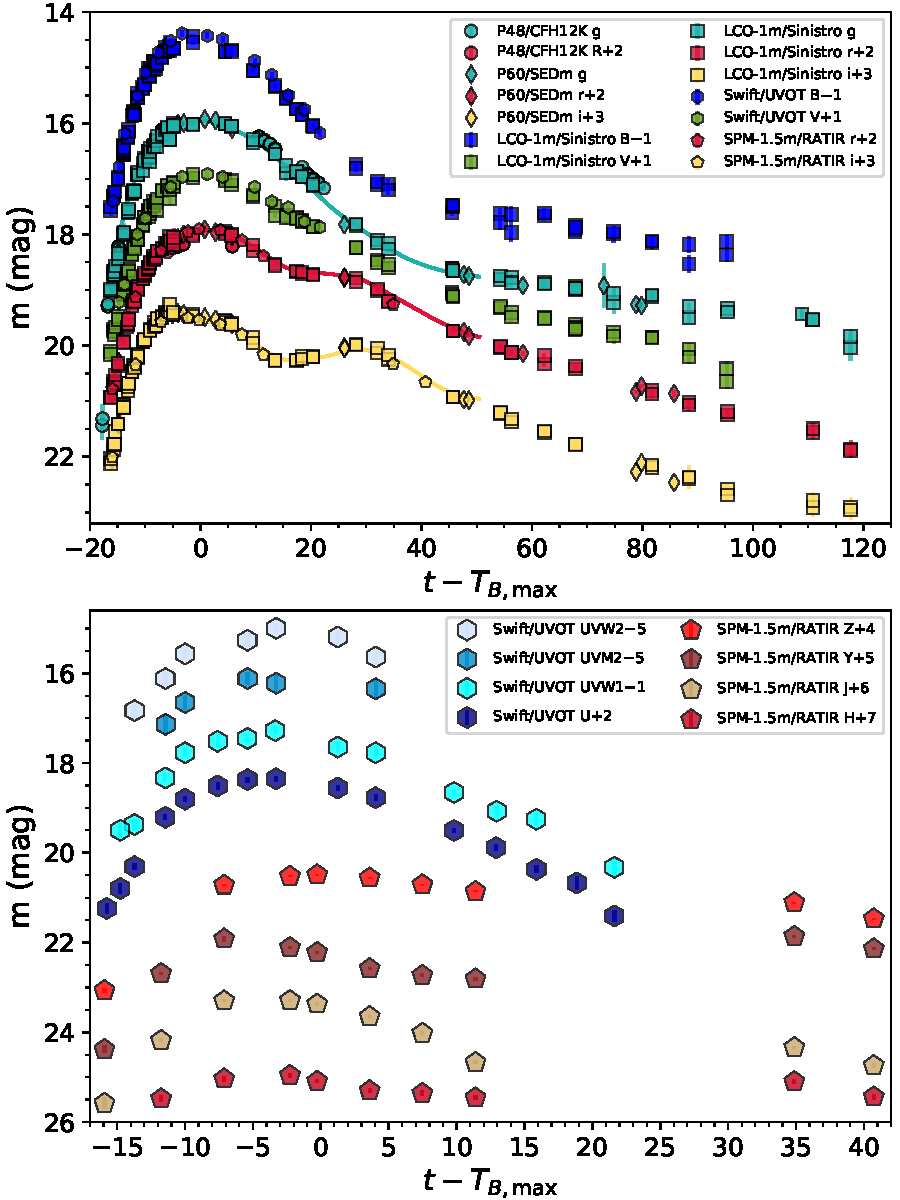
\includegraphics[width=0.95\textwidth]{lightcurve.pdf}
  \caption{Multi-band light curves of iPTF16abc. Each filter is
  represented with a different color, and each instrument with a 
  different symbol. $t_{max}$ is the time of B-band maximum
    determined by SALT2 (Section \ref{sec:classification}). The solid
    curves are best-fit results from SALT2. The black ticks near the
    top of the figure show epochs of spectroscopic observations.}
  \label{fig:lightcurve}
\end{figure*}

During the spring of 2016, the iPTF survey observed the field of iPTF16abc every night in either the $g$- or $R$-band.
Survey observations were conducted with the
CFH12K camera \citep{2000SPIE.3965...58S} on the Palomar Observatory 48-inch telescope 
 (P48). Images were processed by the IPAC image
subtraction and discovery pipeline which subtracts off the background
galaxy light with stacked pre-SN images and performs forced
point-spread-function (PSF) photometry at the location of the SN.\ycao{Add a reference to Frank's PTFIDE paper - http://iopscience.iop.org/article/10.1088/1538-3873/129/971/014002/pdf} The
photometry is then calibrated to the PTF photometric catalog
\citep{2012PASP..124..854O}.

After discovery, photometric observations in the $g'$, $r'$ and $i'$
filters were obtained with the SED Machine 
(SEDM; \ycao{REF}) mounted on the Palomar Observatory 
60-inch telescope (P60). We utilized the Fremling Automated Pipeline \citep{2016A&A...593A..68F} to subtract galaxy light from the SEDM images using achival Sloan Digital Sky Survey (SDSS) images as reference images. This pipeline then performed forced-PSF photometry at the location of iPTF16abc, which is calibrated to the SDSS catalog \ycao{which DR?}.

photometric observations in the \textit{BVgri} were conducted by the Las Cambres Observatory Global Network (LCOGT) 1-m
telescope network.  PSF photometry was measured on these images using
the \texttt{lcogtsnpipe} pipeline \citep{2016MNRAS.459.3939V}. The
\textit{BV} magnitudes are calibrated to the Fourth USNO CCD
Astrograph Catalog \citep{2013AJ....145...44Z}, and the \textit{gri}
magnitudes are calibrated to SDSS Data Release 6
\citep{2008ApJS..175..297A}.

In space, \textit{Swift} observed iPTF16abc on 14 epochs, beginning $\sim$15 d pre-maximum light through $\sim$5 d post maximum. \ycao{check and confirm numbers} The SN flux is measured via aperture photometry on Ultraviolet-Optical
Telescope (UVOT) images via the usual procedures in the HEASoft, including corrections for the coincident loss and aperture loss. The image counts
are converted to physical fluxes using the latest calibration
\citep{2011AIPC.1358..373B}. There are no pre-SN UVOT images at the SN location available in the \textit{Swift} archive.  Visual inspection of the
UVOT images suggests negligible host-galaxy contamination in our UVOT flux measurements. There is no X-ray emission detected at the 
SN position by the \textit{Swift} X-ray Telescope (XRT).

The multi-color light curves of iPTF16abc are illustrated in 
Figure~\ref{fig:lightcurve}.  For convenience, magnitudes in \textit{all}
filters are in the AB system with a zero point of $3631$\,Jy.

Spectroscopic observations of iPTF16abc were undertaken with a variety
of telescopes and instruments in multiple epochs spanning from a
couple of days after explosion to two months after $B$-band maximum. An
observing log is listed in Table \ref{tab:spec_obs_log}. The spectra were reduced using standard routines in \texttt{IDL}/\texttt{Python}. The optical
spectral evolution of iPTF16abc is illustrated in Figure
\ref{fig:spec_seq}, which excludes high-resolution Very Large Telescope (VLT) spectra for clarity.

\begin{deluxetable*}{cccccc}
  \tablecaption{Spectroscopic observations of iPTF16abc \label{tab:spec_obs_log}}
  \tablehead{
    \colhead{Observation MJD} & \colhead{SN phase} & \colhead{Telescope} &
    \colhead{Instrument} & \colhead{Wavelength Coverage (\AA)}
  }
  \startdata
  $57483.26$ & $-16.4$ & DCT & DeVeny\tablenotemark{1} & $3301$--$7499$ \\
  $57483.88$ & $-15.8$ & Gemini-North & GMOS\tablenotemark{2} & $3800$--$9200$ \\
  $57484.51$ & $-15.1$ & Keck-II & DEIMOS\tablenotemark{3} & $5500$--$8099$ \\
  $57486.51$ & $-13.1$ & Keck-II & DEIMOS\tablenotemark{3} & $5500$--$8099$ \\
  $57488.38$ & $-11.3$ & Keck-I & LRIS\tablenotemark{4} & $3055$--$10411$ \\
  $57489.51$ & $-10.1$ & LCOGT-2m & FLOYDS\tablenotemark{5} & $3301$--$8999$ \\
  $57490.40$ & $ -9.3$ & LCOGT-2m & FLOYDS\tablenotemark{5} & $3301$--$9999$ \\
  $57491.55$ & $ -8.1$ & LCOGT-2m & FLOYDS\tablenotemark{5} & $3300$--$9998$ \\
  $57492.20$ & $ -7.5$ & VLT & X-shooter\tablenotemark{6} & $3300$--$24550$ \\
  $57494.00$ & $ -5.7$ & VLT & UVES\tablenotemark{7} & \\
  $57503.32$ & $ +3.7$ & LCOGT-2m & FLOYDS\tablenotemark{5} & $3300$--$9999$ \\
  $57506.00$ & $ +6.3$ & NOT & ALFOSC\tablenotemark{8} & $3602$--$8098$ \\
  $57508.27$ & $ +8.6$ & LCOGT-2m & FLOYDS\tablenotemark{5} & $3301$--$9999$ \\
  $57518.42$ & $+18.8$ & Keck-I & LRIS\tablenotemark{4} & $3071$--$10208$ \\
  $57520.03$ & $+20.4$ & VLT & X-shooter\tablenotemark{6} & $3300$--$24789$ \\
  $57529.40$ & $+29.8$ & LCOGT-2m & FLOYDS\tablenotemark{5} & $4000$--$8998$ \\
  $57542.41$ & $+42.8$ & LCOGT-2m & FLOYDS\tablenotemark{5} & $4000$--$8998$ \\
  $57550.40$ & $+50.8$ & LCOGT-2m & FLOYDS\tablenotemark{5} & $4001$--$8999$ \\
  $57562.38$ & $+62.7$ & LCOGT-2m & FLOYDS\tablenotemark{5} & $4800$--$9300$ \\
  \enddata
  \tablenotetext{1}{The Deveny Spectrograph \citep{2014SPIE.9147E..2NB}}
  \tablenotetext{2}{The Gemini Multi-Object Sectrograph \citep{2004PASP..116..425H}}
  \tablenotetext{3}{DEep Imaging Multi-Object Spectrograph \citep{2003SPIE.4841.1657F}}
  \tablenotetext{4}{Low-Resolution Imaging Spectrometer \citep{1995PASP..107..375O}}
  \tablenotetext{5}{FLOYDS \url{https://lco.global/observatory/instruments/floyds}}
  \tablenotetext{6}{X-shooter \citep{XShooter}}
  \tablenotetext{7}{Ultraviolet and Visual Echelle Spectrograph \citep{2000SPIE.4008..534D}}
  \tablenotetext{8}{The Andalucia Faint Object Spectrograph and Camera \url{http://www.not.iac.es/instruments/alfosc}}
\end{deluxetable*}

\begin{figure*}[!htb]
  \centering
  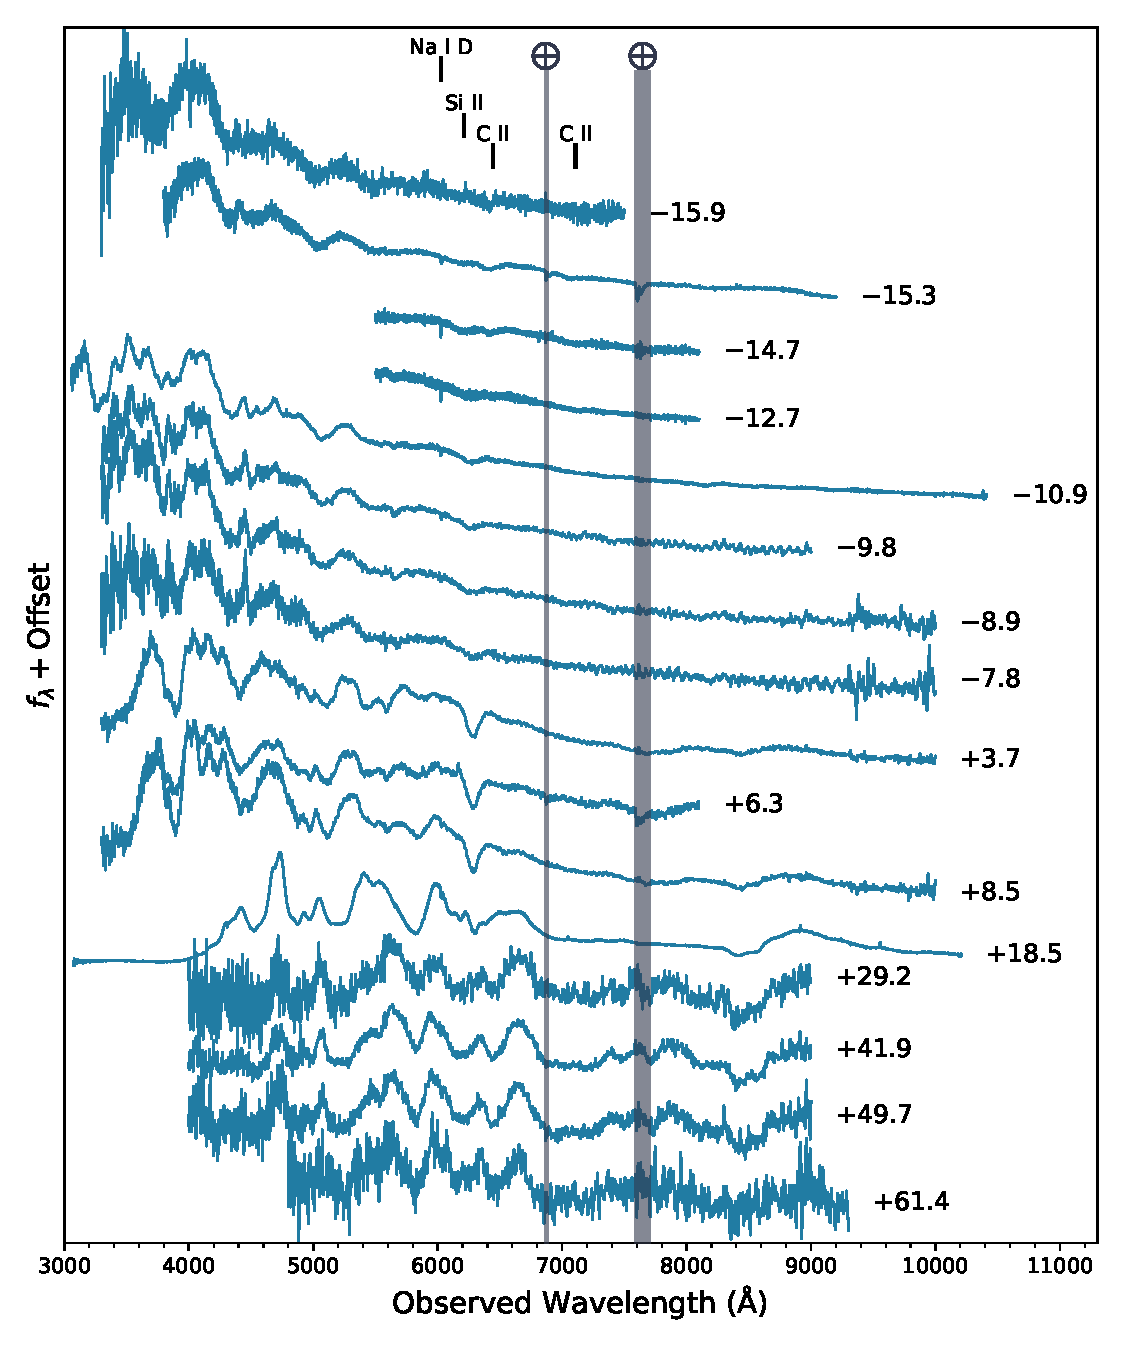
\includegraphics[width=1.0\textwidth]{spectra.pdf}
  \caption{Low-resolution spectra of iPTF16abc are shown in the
    chronical orders. In order for better illustration, each spectrum
    is normalized by the median flux value between $6,000$ and
    $7,000\,\textrm{\AA}$ and offset properly.  The phases in units of
    days are noted next to corresponding spectra. Telluric absorption
    bands are grayed out. The narrow \ion{Na}{1}\,D absorption is also
    highlighted in orange.}
  \label{fig:spec_seq}
\end{figure*}


\section{Reddening, Classification and Host Galaxy}
\label{sec:usual_staff}

\subsection{Reddening}
\label{sec:reddening}

The foreground Galactic extinction toward iPTF16abc
is $E(B-V)=0.0279\,\mathrm{mag}$ \citep{2011ApJ...737..103S}.

Our highest-resolution spectrum of iPTF16abc, obtained with VLT/UVES, shows multiple absorption components for each of the individual lines in the \ion{Ca}{2}\,H$+$K and \ion{Na}{1}\,D doublets (Figure \ref{fig:narrow_features}). This indicates there are two sources of absorption along the line of sight. Fitting
two Gaussian kernels to each line of the \ion{Na}{1} doublet
simultaneously leads to redshifts of $0.02313820\pm0.00000032$ and
$0.02322408\pm0.00000033$. The total \ion{Na}{1}\,D equivalent width (EW) is $0.595\pm0.009\,\textrm{\AA}$ and
$0.609\pm0.008\,\textrm{\AA}$, respectively. Using the empirical
relation between the EW of \ion{Na}{1}\,D lines and
reddening $E(B-V)$ \citep{2012MNRAS.426.1465P}, we derive
$E(B-V)=0.361\pm0.025\textrm{mag}$. We note that this relation has large scatter.

In the VLT/X-shooter spectra of iPTF16abc, we also identify narrow \ion{K}{1}\,7665\,\AA\ and 7699\,\AA\ absorption at the same
redshifts. The double-absorption profiles of \ion{Ca}{2}
and \ion{Na}{1} are not resolved in the VLT/X-shooter spectra. Furthermore, the X-shooter spectra do not show the diffusive
interstellar band at 5780\,\AA. For iPTF16abc, \ion{Na}{1}\,D provides the best estimate of host-galaxy reddening (though see \citealt{2013ApJ...779...38P} for a discussion on why \ion{Na}{1}\,D is a poor tracer of redenning).

\begin{figure}[htb]
  \centering
  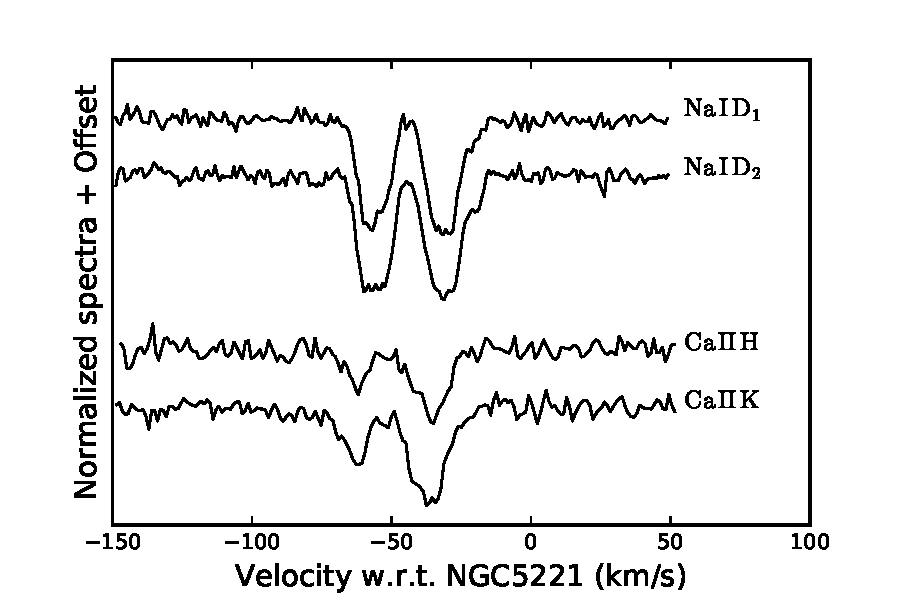
\includegraphics[width=0.45\textwidth]{narrow_abs_features.pdf}
  \caption{Narrow absorption lines of iPTF16abc are shown in this
    figure. The zero velocity corresponds to the redshift of the
    apparent host NGC\,5221.}
  \label{fig:narrow_features}
\end{figure}

We detect \ion{Na}{1}\,D in multiple spectra both before and after peak. After accounting for differing instrumental resolutions, we do not detect any obvious variations in the \ion{Na}{1}\,D profiles.

Finally, we note that the \ion{Ca}{2}\,H$+$K absorption profile is quite different from the \ion{Na}{1}\,D profile. 
This suggests that the dust composition may differ in the two absorption components. 

\subsection{Classfication}
\label{sec:classification}

Using the Supernova Identification (SNID; \citealt{2007ApJ...666.1024B}) package, 
we find the low-resolution spectrum of iPTF16abc at $+18.8$ d is best matched by normal SNe Ia. Several characteristic features of a SN
Ia, such as \ion{Si}{2}, \ion{S}{2}, can be easily identified in the
spectra of iPTF16abc (Figure \ref{fig:spec_seq}).

To determine the brightness and time of $B$-band maximum for 
iPTF16abc, we fit the P60 light curves with the \texttt{sncosmo} software package.\footnote{The
  \texttt{sncosmo} Python module is available at
  \url{https://sncosmo.readthedocs.io/en/v1.5.x/}.} This fit includes a SALT2 template \citep{2007A&A...466...11G} modified by the line-of-sight extinction
curve \citep{1999PASP..111...63F} with $E(B-V)$ values from Section
\ref{sec:reddening} and $R_V=3.1$.

We determine the time of rest-frame \textit{B}-band maximum to be 
 $\textrm{MJD}_{max}=57499.54\pm0.23$, the coefficient
of the zeroth principle component $x_0 = XXX \pm XXX$, the
coefficient of the first principle component $x_1 = 0.9655 \pm 0.0003$, and
the color term $c = 0.012 \pm 0.029$. The best-fit model also gives an
unreddened apparent peak magnitude of $m^*_{B}=15.6\,\textrm{mag}$ \ycao{uncertainties on Bmax?} in
the SN rest frame.

For convenience, in the following sections, we define the best-fit
value $\textrm{MJD}_{max}=57499.54$ as phase $t=0$.

\subsection{Host Galaxy}
\label{sec:host}

After establishing iPTF16abc as a normal SN Ia, we use the latest
calibration \citep{2014A&A...568A..22B} of the Phillips relation
\citep{1993ApJ...413L.105P} using $m^*_{B}$, $x_1$ and $c$ to derive a
distance modulus $\mu = 34.72 \pm 0.09 \,\textrm{mag}$ to the SN, provided
that the host galaxy of iPTF16abc has a stellar mass less than
$10^{10}\sm$. We note that a more massive host galaxy would result in a larger inferred distance modulus that is nevertheless consistent within the uncertainties.

The location of iPTF16abc is spatially coincident with a tidal tail of
galaxy NGC\,5221. \citet{2007A&A...465...71T} derived a distance
modulus of $35.0\pm0.4\,\textrm{mag}$ to NGC\,5221 from the Tully-Fisher
relation. This distance modulus is consistent with that of iPTF16abc.

Separately, \citet{1998A&AS..130..333T} observed the 21-cm line in
this galaxy and measured a redshift of $0.0233303\pm0.000027$.  The
two components in the \ion{Na}{1}\,D have a relative velocity of
$-57.6\pm8.1\,\textrm{km}\,\textrm{s}^{-1}$ and
$-31.8\pm8.1\,\textrm{km}\,\textrm{s}^{-1}$, suggesting that both
absorption resources are probaly located on the tidal tail of
NGC\,5221.\ycao{This is confusing - are those velocities relative to host redshift or LSR?}


\section{First Light And Explosion Time}
\label{sec:first_light}

\subsection{Light Curve Fit}
\label{sec:lc_fit}

The time of first light for SNe is usually estimated by 
extrapolating early-phase light curves to match simple 
mathematical models. Assuming an ideal exapnding fireball with 
constant temperature, \citet{1982ApJ...253..785A} derives that $f 
\propto t^2$, where $f$ is the SN flux and $t$ is the time since 
explosion. To account for variations of the photospheric 
temperature during expansion, we model the early light curve as a power law:
\begin{equation}
  \label{eq:broken_power_law}
  f(t) \left\{
    \begin{array}{ll}
      = 0,\ \textrm{when}\ t<t_0 \\
      \propto (t-t_0)^{\alpha},\ \textrm{when}\ t>t_0
    \end{array}
  \right.\ ,
\end{equation}
where $t_0$ is the time of first light and $alpha$ is the power-law index. We limit our fit to the earliest detections of iPTF16abc, which were exclusively in $g$-band. To determine the best fit parameters, we search a large grid over $t_0$, $\alpha$
and the proportionality constant, and minimize $\chi^2$. 
We note that the definition of
the time window for the early light curve may affect the fitting
result, so we experiment the fitting procedure with different time
windows. \ycao{I don't understand what this previous sentence means}
The modeling results show that the SN flux rises approximately
linearly between
$t=-19\,\textrm{d}$ and $t=-15\,\textrm{d}$. Figure \ref{fig:early_lc_fit} shows the best-fit result and
the joint marginal distribution of $t_0$ and $\alpha$. With the
best-fit model of $\alpha=0.92$ and $t_0=-18.47$ days, our first
detection of iPTF16abc was made only $\sim{0.2}\,\textrm{d}$ after 
the SN first light. From the fit, we additionally infer a total rise time to \textit{B}-band peak of $18.47$
days.

\begin{figure*}[htb]
  \centering
  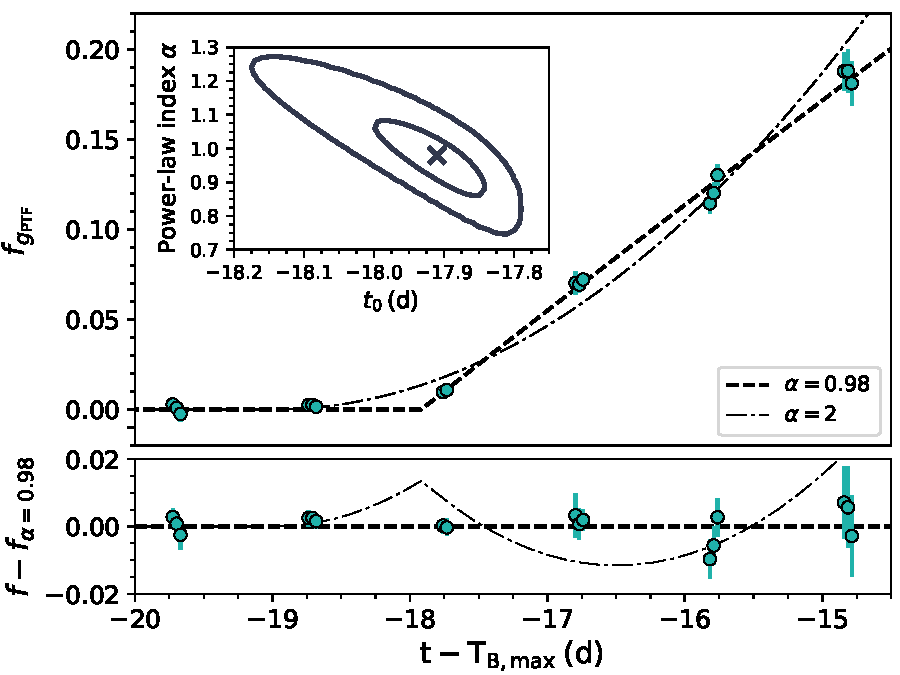
\includegraphics[width=0.95\textwidth]{early_lc.pdf}
  \caption{Broken Power low fitting to the early $g$-band light
    curve. The best-fit model of $\alpha=0.92$ and $t_0=-18.47\,\textrm{days}$
    and corresponding residues are shown in the top and bottom panels, respectively.
    The joint distribution of $t_0$ and $\alpha$ is illustrated in the inset of
    the upper panel. The solid and dashed contours represent the $68\%$ and $99.7\%$
    confidence levels.
  }
  \label{fig:early_lc_fit}
\end{figure*}

Starting around $t=-15\,\textrm{d}$, the $g$-band light curve 
deviates from the above best-fit model and 
rises significantly faster, indicating a
change in the power-law index $\alpha$. In fact, between $t=-14\,\mathrm{d}$ and $t=-8\,\mathrm{d}$ the light curve is well fit by a power law of index $1.40$. In other words, the entire light curve
before $t=-8$\,days can be approximated by a broken power-law model
(e.g.,
\citealt{2013ApJ...778L..15Z,2014ApJ...783L..24Z,2016arXiv161202097Z,
  2016arXiv161202725Z}).

As discussed in Section \ref{sec:lc_energy}, the initial light curve
of iPTF16abc is probably purely powered by the radioactive decay of
$^{56}$Ni. Thus, the initial rise of the light curve depends on
the depth of the shallowest layer where $^{56}$Ni is deposited
\citep{2014ApJ...784...85P}. According to theoretical mdels
\citep{2016ApJ...826...96P}, the linearly rising light curve implies
strong mixing of $^{56}$Ni in the ejecta. As a result, the time lag
between the time of explosion and SN first light is negligible.

\subsection{Expansion Velocity Fit}
\label{sec:early_vel}

Due to the possibility of an early dark phase for SNe Ia, \citet{2014ApJ...784...85P} suggest that photospheric velocity measurements be used to determine the time of explosion, because the ejecta expand from the onset of the SN explosion. Assuming a
constant opacity in the ejecta, \citeauthor{2014ApJ...784...85P} find that the photospheric velocity evolves as
$v_{ph}\propto(t-t_{exp})^{-0.22}$. While the photospheric velocity
is not easy to measure, line velocities of \ion{Si}{2} or \ion{Ca}{2}
can be used as a proxy
\citep{2014ApJ...784...85P,2016ApJ...826..144S}.

In the case of iPTF16abc, the \ion{Ca}{2} IR triplet is very weak, 
probably due to high ejecta temperature. Thus, we
determine the photospheric velocity from the \ion{Si}{2}\,6355 line. Visual
inspection shows no sign of multi-velocity components
of \ion{Si}{2}, and that the \ion{C}{2}\,6580 line overlaps the red
wing of the \ion{Si}{2} line. Consequently, we model the observed 
spectra between $5,900$ and $6,500$\,\AA (rest-frame)
with two gaussian kernels superposed on a linear baseline, which
accounts for \ion{Si}{2}, \ion{C}{2} and the
continuum, respectively. The expansion
velocity of \ion{Si}{2} is measured by the central wavelength
of the \ion{Si}{2} Gaussian kernel.

\begin{figure*}[!thb]
  \centering
  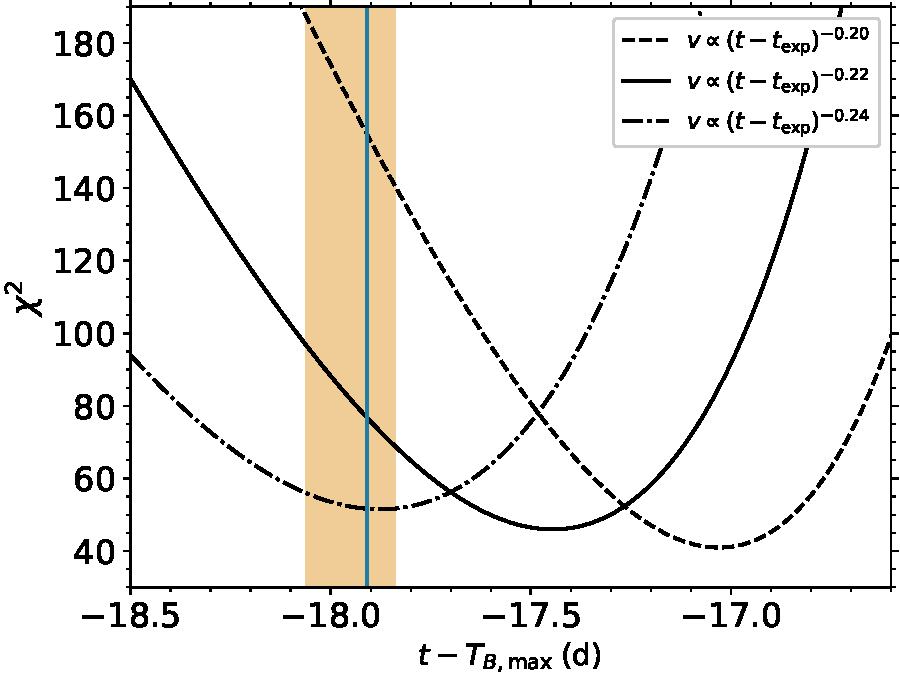
\includegraphics[width=0.45\textwidth]{Chi2.pdf}
  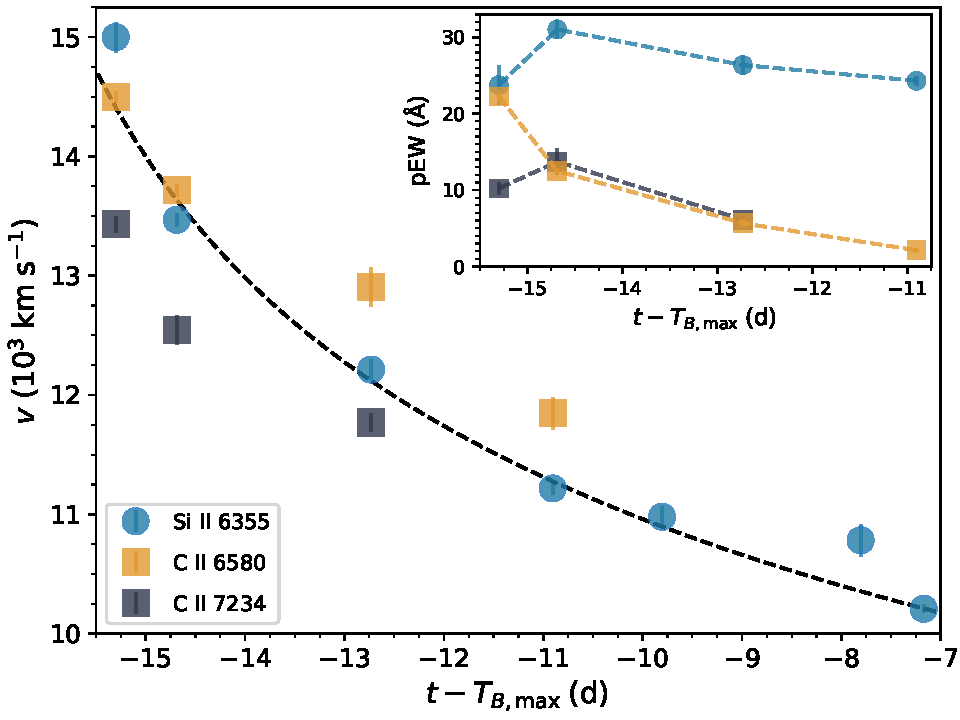
\includegraphics[width=0.45\textwidth]{VelocityPlot.pdf}
  \caption{Constraints on $t_{exp}$ from fitting the velocity
    evolution of \ion{Si}{2}.
    \textit{Left panel:} the dashed, solid
    and dash-dotted curves show $\chi^2$ for fitting power laws with
    indices $-0.20$, $-0.22$ and $-0.24$, respectively. The red
    vertical line and the orange region indicate $t_0$ and its
    3-$\sigma$ confidence interval from Section
    \ref{sec:lc_fit}.
    \textit{Right panel:} Observed \ion{Si}{2}\,6355
    velocities and the best-fit power-law velocity with an index of
    $-0.22$.}
  \label{fig:velocity_t_exp}
\end{figure*}

We fit the measured velocities of \ion{Si}{2}\,6355 line to the
$v\propto(t-t_{exp})^{-0.22}$ model by minimizing the $\chi^2$ value
and find the best-fit explosion time $t_{exp}=-17.95\,\textrm{days}$
with a 3-$\sigma$ confidence interval between $-17.4\,\textrm{days}$
and $-18.3\,\textrm{days}$ (Figure \ref{fig:velocity_t_exp}). We additionally
alter the power-law index to $-0.20$ and $-0.24$ to examine the
sensitively of the result on the assumed power-law index.  This 
leads to consistent results within the respective 3-$\sigma$ 
confidence intervals.

Compare the estimated $t_{exp}$ to $t_0$ (left panel of Figure
\ref{fig:velocity_t_exp}), we find that $t_0\lessapprox t_{exp}$.\footnote{Note that the uncertainties on $t_{exp}$ are large due to assumptions in the $v\propto(t-t_{exp})^{-0.22}$ model.}
Since physical causality requires $t_{exp}<t_0$, we draw the qualitative
conclusion that $t_0\simeq t_{exp}$, which is consistent
with our inference from the early light curve analysis (Section
\ref{sec:lc_fit}).

From $t_{exp}$, we estimate the actual rise time of iPTF16abc from the
time of explosion to \textit{B}-band maximum to be $17.95$ d.  In
comparison, SN2011fe has $t_0=-17.7$ d \citep{2013A&A...554A..27P}
with a preceding dark period of $\sim 1$ day
\citep{2014ApJ...784...85P}. ASASSN-14lp has $t_0=-16.94$ days with a
preceding dark period of about acouple of days
\citep{2016ApJ...826..144S}. This comparison suggests that the actual
rise time of a SN Ia between the SN explosion and the \textit{B}-band
maximum is roughly a constant, which largely depends on the total mass
of synthesized $^{56}$Ni.\ycao{I am not convinced by this last sentence}

\subsection{Strong and Short-Lived Carbon Features}
\label{sec:carbon}

iPTF16abc exhibits unusually strong absorption of
\ion{C}{2} $\lambda\lambda$6580, 7234 for SNe Ia. Our analysis of the
\ion{Si}{2}\,6355 line also allows us to measure the velocities and
pseudo-equivalent widths (pEWs) of \ion{C}{2}\,6580. We also fit a Gaussian
kernel with linear baseline to the spectral region near
the \ion{C}{2}\,7234 line to measure its velocity and pEW. 
The velocity evolution of \ion{C}{2} is shown in the right panel
of Figure \ref{fig:velocity_t_exp} and the pEW evolution
in Figure \ref{fig:ew}. 

Our measurements show that the strong \ion{C}{2} absorption
only appears in the very early phases. In the spectrum taken at
$t=-15.8$ days, the pEW of \ion{C}{2}\,6580 is comparable to that
of \ion{Si}{2}\,6355. Subsequent spectra the pEW of \ion{C}{2} 
decreases until the feature is no longer detectable 
around $t=-10$ days. 

\begin{figure}[!htb]
  \centering
  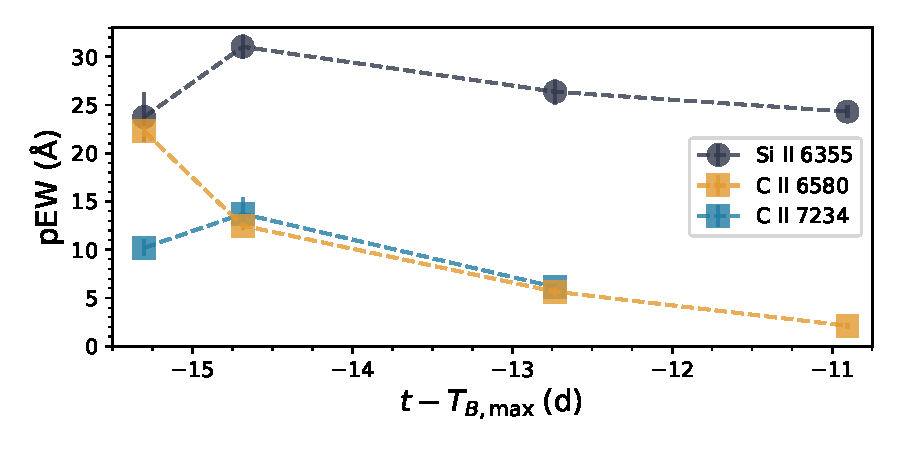
\includegraphics[width=0.45\textwidth]{pEW.pdf}
  \caption{Pseudo-equivalent width of \ion{Si}{2}\,6355,
    \ion{C}{2}\,6580 and \ion{C}{2}\,7234 lines. The uncertainties
    in these measurements are less than the sizes of these symbols.}
  \label{fig:ew}
\end{figure}

\ion{C}{2} absorption requires the existence of both unburned
carbon and $^{56}$Ni, which radioactively decays and ionizes the C 
atoms. The strong and short-lived \ion{C}{2} features reveal 
that $^{56}$Ni atoms have been strongly mixed in to the outter 
layers of the ejecta. This provides a third piece of evidence
for strong mixing in the iPTF16abc ejecta. 

Carbon signatures are seen in $> 1/4$ of all normal SNe Ia before
maxima
\citep{2011ApJ...732...30P,2012MNRAS.425.1917S,2011ApJ...743...27T},
but the signatures are usually weak. Even in SN2011fe, which was discovered and spectroscopically observed shortly after explosion, the \ion{C}{2}
features are not strong in the first spectra
\citep{2012ApJ...752L..26P}.  The only normal SN Ia known to have
strong \ion{C}{2} features at early phases is SN2013dy
\citep{2013ApJ...778L..15Z}. Unlike iPTF16abc, however, the pEWs 
of the \ion{C}{2} features in SN2013dy are \ycao{not?} as large as 
those of \ion{Si}{2}\,6355 in the same spectra.


\subsection{Discussion}
\label{sec:lc_energy}

Multiple energy sources can contribute to the early radiation from a SN Ia: SN shock
breakout, SN ejecta-companion collision, and radioactive 
$^{56}$Ni. The previous analysis is based on the assumption that the light curve of
iPTF16abc is powered purely by radioactive decay. Here we discuss the
other two possibilities.

\subsubsection{SN Shock Breakout}

The shock breakout of a SN Ia lasts for a fraction of a second due to
the small size of the exploding star. However, the subsequent cooling
phase may last longer (e.g., \citealt{2010ApJ...708..598P}).
Following the analysis of SN2011fe in \citet{2012ApJ...744L..17B}, we
compare the early-phase \textit{g}-band light curve of iPTF16abc with
two cooling models \citep{2011ApJ...728...63R, 2010ApJ...708..598P}. From this comparison, we limit the radius of 
the
progenitor of iPTF16abc to be $<1\sr$, which is a weak constraint compared to SN~2011fe. Assuming a 
typical white-dwarf radius for the progenitor, $\sim{0.01}\sr$, the cooling emission of a
SN Ia is negligible at the time of our first iPTF16abc detection. 
Thus, we conclude that shock cooling does not contribute to the 
early light from iPTF16abc.

\subsubsection{SN-Companion collision}

SNe Ia with single-degenerate progenitors can produce detectable 
radiation following the collision of the SN ejecta with the 
non-degenerate companion. Geometrically the odds of such a 
detection are low, however, at $\sim$10\%. According to 
calculations by
\citet{2010ApJ...708.1025K}, SN ejecta-companion star collisions 
generate thermal emission with a spectrum that peaks in the 
ultraviolet. Thus, any resulting \textit{g}-band emission is very weak.

To examine the possibility of a SN-companion signature in the early
light curve of iPTF16abc, we employ the \citet{2010ApJ...708.1025K}
model and assume an ejecta mass of $1.4\sm$, an expansion velocity of
$10^{4}\,\textrm{km}\,\textrm{s}^{-1}$, and a constant opacity of
$0.2\,\textrm{cm}^2\,\textrm{g}^{-1}$. The angular dependence of this
emission uses the parameterized equation in
\citet{2012ApJ...749...18B}.  Figure \ref{fig:SN-companion} compares
the expected \textit{g}-band apparent magnitudes of SN-companion
collisions for different binary separation assuming the optimal viewing
angle against the first detection of iPTF16abc. The figure shows that,
even with the most favorable viewing angle, the binary separation would
have to exceed $2\times10^{14}\,\textrm{cm}$. Under the model assumption that the
companion fills its Roche lobe, the companion star would have to have
a radius of $\sim10^{14}\,\textrm{cm}\simeq10 \mathrm{AU}$. Given that the
mass of the companion is $\sim1\sr$, such a large radius is unphysical.
Therefore, we conclude that the early emission of iPTF16abc is not 
due to a collision between the eject and a non-degenerate companion.

\begin{figure}[!thb]
  \centering
  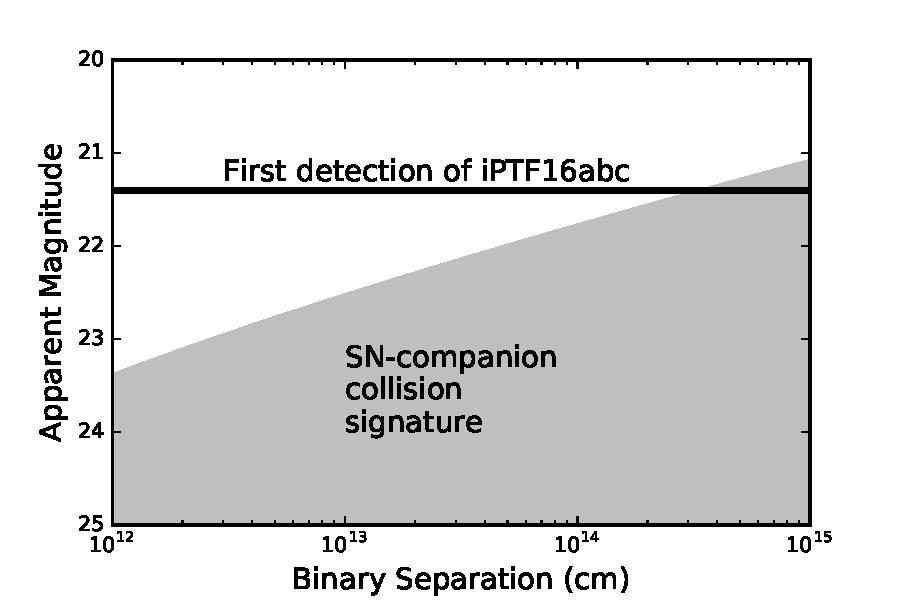
\includegraphics[width=0.45\textwidth]{SNCompanion.pdf}
  \caption{Apparent magnitude of a SN-companion collision (gray region)
    against the first detection of iPTF16abc (black).}
  \label{fig:SN-companion}
\end{figure}

\section{Conclusion}
\label{sec:conclusion}

We have presented observations of the extraordinarily early discovery of the 
normal Type Ia supernova iPTF16abc. Our fast-response follow-up 
compaign allowed us to draw the following conclusions:
\begin{itemize}
\item By extrapolating the early light curve, we determined that the
  SN first light occured only $\sim{0.2}$ d before our
  first detection.
\item Our analysis showed that the observed early-phase light curve is
  probably powered by $^{56}$Ni radioactive decay. We find no 
  evidence for detectable signatures of SN
  shock breakout or SN ejecta-companion collision (provided that 
  iPTF16abc
  is born in a single-degenerate channel).
\item Our measurements of the spectral line velocities show that the
  SN explosion date is approximately equal to the time
  of the first light. This indicates that
  synthesized $^{56}$Ni atoms are strongly mixed into the 
  outer layers of
  the supernova ejecta.
\item The strong and short-lived carbon features seen in the 
  earliest spectra of iPTF16abc provide additional evidence
  for strong $^{56}$Ni mixing in the SN ejecta.  
\end{itemize}

Extremely early observations of young SNe provide a ``smoking
gun'' to probe the mixing level in the ejecta, which, in turn, is 
a result of the explosion mechanism. Ongoing and planned
time-domain surveys will discover a large number of very young supernovae over the next few years. As this sample grows, we will
be able to make connections between the observed SN properties and 
proposed explosion mechanisms.

Finally, we close by emphasizing the importance of fast-response photometric and spectroscopic follow-up campaigns. Without the early recognition of the youth of this SN and the associated follow-up, much of the analysis presented herein would not have been possible. Moving forward, the ability to trigger such observations is essential to improve our understanding of the physics of SNe Ia.

\acknowledgements

YC thanks supports from the postdoc fellowship in the eScience
institute, University of Washington.

\bibliographystyle{aasjournal}
\bibliography{ref}

\end{document}
